% Main LaTeX file for the thesis/project report
\documentclass[12pt,a4paper]{report}

% Encoding and language
\usepackage[utf8]{inputenc}
\usepackage[T1]{fontenc}
\usepackage{lmodern}
\usepackage[english]{babel}

% Page and typography
\usepackage{geometry}
\geometry{margin=1in}
\usepackage{setspace}
\onehalfspacing
\usepackage{microtype}

% Figures, tables, colors
\usepackage{graphicx}
\usepackage{caption}
\usepackage{subcaption}
\usepackage{booktabs}
\usepackage{multirow}
\usepackage{xcolor}

% Math
\usepackage{amsmath, amssymb, amsfonts}

% Hyperlinks
\usepackage[hidelinks]{hyperref}

% Bibliography
\usepackage[numbers,sort&compress]{natbib}

% If available, allow including webp logos; otherwise fall back to png/pdf
% (README explains conversion if needed)
\newcommand{\unilogo}{project_report/logo/ru_logo}

% Title data
\newcommand{\reporttitle}{Benchmarking Attention for Ocular Disease Classification: EfficientNet vs CBAM on ODIR\textendash 5K}
\newcommand{\supervisor}{Dr. Md. Matiqul Islam}
\newcommand{\authors}{Md. Takrim\textendash Ul\textendash Alam\\ Samiul Bashir}
\newcommand{\department}{Department of Information and Communication Engineering}
\newcommand{\university}{University of Rajshahi}
\newcommand{\reportdate}{\today}

\begin{document}

% Title page
\begin{titlepage}
  \centering
  % Try webp, then png, then pdf
  \IfFileExists{\unilogo.webp}{\includegraphics[width=0.25\textwidth]{\unilogo.webp}\\[1em]}{%
  \IfFileExists{\unilogo.png}{\includegraphics[width=0.25\textwidth]{\unilogo.png}\\[1em]}{%
  \IfFileExists{\unilogo.pdf}{\includegraphics[width=0.25\textwidth]{\unilogo.pdf}\\[1em]}{}}}
  {\LARGE \university\\[0.3em] \department\par}
  \vspace{2cm}
  {\huge\bfseries \reporttitle\par}
  \vspace{1.5cm}
  {\Large \textbf{Supervisor:} \supervisor\par}
  \vspace{0.8cm}
  {\Large \textbf{Authors:}\\ \authors\par}
  \vfill
  {\Large \reportdate\par}
\end{titlepage}

\pagenumbering{roman}
\tableofcontents
\listoffigures
\listoftables
\clearpage

\pagenumbering{arabic}

% Abstract
\section*{Abstract}
This project investigates attention mechanisms for ocular disease classification using fundus images from the ODIR\textendash 5K dataset. We compare a strong convolutional baseline (EfficientNet) against an attention\textendash augmented variant employing the Convolutional Block Attention Module (CBAM). Our pipeline parses ODIR metadata, prioritizes Hypertension labeling where present, and enforces robust stratified splits to ensure all target classes appear in validation and test sets. Experiments demonstrate that image\textendash specific attention improves several classes, while Hypertension remains challenging due to limited single\textendash label prevalence and ambiguity in diagnosis text. We provide full training/evaluation artifacts (curves, confusion matrices, and metrics) to support reproducibility and future extensions, including multi\textendash label learning and targeted augmentation for rare classes.



% NOTE: The main topic names below should be aligned to the prior year's Table of Contents.
% Replace the section headings if your department requires exact titles.

% 1. Introduction
\chapter{Introduction}
Retinal fundus photography provides a non\textendash invasive window into ocular health, enabling screening and diagnosis for conditions such as Glaucoma (G), Cataract (C), Age\textendash related Macular Degeneration (AMD, A), Hypertension\textendash related retinopathy (H), and Myopia (M). Automated classification can assist clinicians by prioritizing high\textendash risk cases and scaling screening programs.

Deep convolutional networks (CNNs) learn strong visual features but can struggle with class imbalance, domain variability, and subtle disease cues. Attention mechanisms explicitly reweight feature channels and spatial regions, potentially improving discrimination on small or ambiguous lesions. In this project we evaluate an EfficientNet baseline and an EfficientNet+CBAM variant on ODIR\textendash 5K, following a robust data parsing and splitting procedure, and report comprehensive metrics and plots to support a fair comparison.

\section{Contributions}
\begin{itemize}
  \item A practical ODIR\textendash 5K pipeline with robust parsing and Hypertension\textendash priority labeling to mitigate label sparsity in validation/test.
  \item An attention\textendash enhanced classifier (EfficientNet+CBAM) compared against a matched EfficientNet baseline under identical preprocessing, augmentation, and training schedules.
  \item Thorough evaluation artifacts (training curves, confusion matrices, ROC/PR curves, macro/weighted F1, ROC\textendash AUC and PR\textendash AUC) prepared for report integration.
\end{itemize}


% 2. Related Work
\chapter{Related Work}
\section{Fundus Image Classification}
CNNs such as VGG, ResNet, and EfficientNet have been widely applied to fundus image analysis for diabetic retinopathy screening and broader ocular disease classification. EfficientNet family models leverage compound scaling and strong ImageNet pretraining for competitive performance at modest compute cost \cite{tan2019efficientnet}.

\section{Attention Mechanisms}
Channel and spatial attention mechanisms (SE, CBAM, ECA) improve CNN feature quality by adaptively reweighting salient signals. CBAM applies sequential channel and spatial attention via lightweight modules with minimal overhead \cite{woo2018cbam}. For accessible primers on CBAM and related attention modules, see \cite{cbamMedium, cbamDO}. Vision transformers (ViT) and token\textendash based self\textendash attention have also shown promise, but often require larger datasets or heavy augmentation.

\section{ODIR\textendash 5K and Labeling}
The ODIR dataset provides paired left/right fundus images and metadata. Practical pipelines must reconcile free\textendash text diagnoses to structured labels and contend with multi\textendash label prevalence and class imbalance. Prior work also explored generative augmentation for minority classes.


% 3. Dataset
\chapter{Dataset}\label{sec:dataset}
\section{ODIR\textendash 5K Overview}
We use ODIR\textendash 5K (Kaggle) \cite{odir5k} containing fundus images with metadata. Our study focuses on five target classes: Glaucoma (G), Cataract (C), AMD (A), Hypertension (H), and Myopia (M).

\section{Label Parsing and Hypertension Priority}
Free\textendash text diagnoses are mapped to short codes using keyword matching (e.g., ``hypertensive retinopathy'', ``hypertensive'', ``htn'' $\rightarrow$ H). If Hypertension appears among multiple diagnoses for an eye, we assign the final label as H, otherwise select the first class by a fixed order (G, C, A, H, M). Missing or out\textendash of\textendash scope labels are discarded.

\section{Splits and Preprocessing}
We ensure stratified splits (train/val/test) with all target classes represented in validation and test via repeated StratifiedShuffleSplit attempts. Images are resized to $224\times224$, normalized using EfficientNet preprocessing, and augmented (random flip, small rotation, zoom, and contrast) during training.


% 4. Methodology
\chapter{Methodology}
\section{Baselines and Architecture}
\textbf{EfficientNet Baseline:} ImageNet\textendash pretrained EfficientNetB0 (optionally B3) with a light classification head: BN $\rightarrow$ Conv1x1 (192) $\rightarrow$ GAP $\rightarrow$ Dropout(0.4) $\rightarrow$ Dense(192, ReLU) $\rightarrow$ Dropout(0.4) $\rightarrow$ Softmax.

\textbf{EfficientNet + CBAM:} Same backbone and head, with a CBAM block applied on the convolutional feature map to apply channel and spatial attention.

\section{Training}
Optimizer: Adam (lr $3\times10^{-4}$), batch size 16, warm\textendash up forward pass, callbacks: ModelCheckpoint (best val acc), ReduceLROnPlateau, EarlyStopping. Mixed precision is enabled for memory efficiency.

\section{Evaluation}
We report accuracy, macro/weighted F1, ROC\textendash AUC (macro one\textendash vs\textendash rest), PR\textendash AUC (macro), and confusion matrices. Curves (training/validation for accuracy, loss, ROC\textendash AUC, PR\textendash AUC) and per\textendash class ROC/PR curves are exported.


% 5. Experimental Setup
\chapter{Experimental Setup}
We document the compute environment, training protocol, and hyperparameters shared by both models, alongside exported artifacts that support reproducibility and auditability of results.
\section{Environment}
Experiments run on Kaggle GPU runtimes with TensorFlow/Keras, using mixed precision. A Tesla P100 GPU was used; the end-to-end training and report-generation pass completed in approximately 846.8 seconds. Outputs (plots, confusion matrices, CSVs, and best models) are saved in the session working directory.

Using a standard Kaggle environment maximizes reproducibility: any researcher can access an identical software stack (TensorFlow, Keras, cuDNN) and comparable hardware. The Tesla P100 (16GB VRAM, Pascal) offers a robust baseline. The ~14 minute wall time (846.8s) includes data loading, augmentation, multi\textendash epoch training with early stopping, evaluation, and artifact generation, reflecting an efficient pipeline enabled by mixed precision. High\textendash FLOPS ops run in float16 while numerically sensitive parts (final softmax and loss) remain in float32, providing 2\textendash 3x speedups and halving activation memory, which permits a batch size of 16 for high\textendash resolution inputs.

\paragraph{Model sizes.} Best EfficientNet baseline checkpoint: 87.26 MB. Best EfficientNet+CBAM checkpoint: 91.40 MB. The CBAM module adds a small memory overhead while improving attention quality and per\textendash class separability.

Checkpoints are saved in Keras formats (.h5/.keras). The ~4.14 MB increase in the CBAM variant reflects the added channel MLP (two\textendash layer) and a $7\times7$ spatial convolution. This overhead is negligible for storage and inference, yet it yields the performance gains detailed in Section~\ref{sec:results}.

\section{Protocols and Reproducibility}
We fix random seeds and use stratified splits that ensure all 5 classes appear in validation and test. Preprocessing follows EfficientNet conventions; augmentation includes flips, small rotations, zoom, and contrast. We monitor validation accuracy with early stopping and learning rate reduction. All figures in this paper (training curves, percent confusion matrices, and Grad\textendash CAM panels) are exported by the notebook \cite{takrimNotebook} to support full reproducibility.

We fix global seeds (NumPy, Python \texttt{random}, TensorFlow) to control weight initialization and shuffling, reducing run\textendash to\textendash run variance. Stratified splitting is compulsory on long\textendash tailed data; without it, minority classes (e.g., Hypertension) may vanish from validation/test, corrupting macro F1 and per\textendash class metrics. Preprocessing adheres to EfficientNet input sizing (e.g., $224\times224$ for B0) and normalization. Augmentations (H/V flips, rotations $\pm10^{\circ}$, zoom/contrast $\pm20\%$) are lightweight to encourage learning pathology\textendash relevant features rather than camera artifacts. The linked Kaggle notebook acts as an executable paper, generating all artifacts programmatically for auditability.

\paragraph{Training Protocol Recap.} We use Adam (lr $3\times10^{-4}$), batch size 16, mixed precision, ModelCheckpoint (monitoring val\_acc), ReduceLROnPlateau, and EarlyStopping with best weight restore. Class weights counter imbalance.

ModelCheckpoint selects the best generalizing epoch by validation accuracy. EarlyStopping (e.g., patience=10) halts when validation accuracy stalls, preventing overfitting and wasted compute. ReduceLROnPlateau (e.g., patience=5, factor=0.1) reduces the learning rate after stagnation, enabling finer convergence. Class weights are the inverse frequency of each class in the training split, increasing the loss penalty for rare Hypertension errors relative to common classes.

\section{Hyperparameters}
Batch size 16, epochs up to 40 with early stopping, Adam lr $3\times10^{-4}$, augmentation as in Section~\ref{sec:dataset}. The same schedule is applied to both baseline and CBAM variants.

Batch size 16 saturated the 16GB P100 VRAM under mixed precision, balancing gradient stability and memory. An epoch cap of 40 provides headroom; EarlyStopping typically triggers between epochs 20\textendash 30 as validation accuracy plateaus. Adam at $3\times10^{-4}$ is a conservative fine\textendash tuning rate that preserves ImageNet priors while adapting to fundus imaging. Crucially, hyperparameters are identical across baseline and CBAM to isolate the architectural change as the only independent variable.

\paragraph{Metrics Justification.} Accuracy, macro/weighted F1, ROC\textendash AUC (macro OvR) and PR\textendash AUC (macro) together provide balanced assessment under long\textendash tailed distributions; PR\textendash AUC emphasizes minority sensitivity by focusing on precision\textendash recall.

Accuracy is skewed toward majority classes and is reported for completeness. Macro F1 averages per\textendash class F1, penalizing failures on minority Hypertension commensurately. Weighted F1 reflects support and often tracks accuracy. Macro ROC\textendash AUC (OvR) evaluates threshold\textendash free discriminability per class, then averages. Macro PR\textendash AUC is especially sensitive to minority performance by ignoring true negatives that otherwise inflate ROC\textendash AUC.

\section{Artifacts}
For each model we export: training curves (accuracy, loss, ROC\textendash AUC, PR\textendash AUC), confusion matrices (counts and CSV), classification reports, ROC/PR curves per class, and a metrics summary table to compare variants.

Training curves reveal optimization dynamics and callback triggers. Confusion matrices (counts and row\textendash normalized percent) expose per\textendash class recall and error modes. Classification reports provide per\textendash class P/R/F1 that feed macro/weighted F1. Per\textendash class ROC/PR curves visualize discriminability beyond single thresholds. A metrics summary CSV aggregates scalars for direct baseline vs CBAM comparison. Best model checkpoints (.h5/.keras) support downstream inference and Grad\textendash CAM generation without retraining.

\paragraph{Reproducibility.} The training and evaluation flow is provided in a Kaggle notebook \cite{takrimNotebook}, which produced all figures integrated in Section~\ref{sec:results}.


% 6. Results and Discussion
\chapter{Results and Discussion}\label{sec:results}
\section{Quantitative Comparison}
We compare EfficientNet (no attention) against EfficientNet+CBAM on identical splits. Metrics include accuracy, macro/weighted F1, ROC\textendash AUC (macro OvR), and PR\textendash AUC (macro). Attention improves several classes, while Hypertension remains challenging due to limited single\textendash label prevalence. Class weighting or multi\textendash label learning may further improve H.

As shown in Figure~\ref{fig:train_curves}, both variants converge smoothly; the CBAM model trends to higher validation accuracy and lower loss. Figure~\ref{fig:auc_curves} summarizes ROC\textendash AUC and PR\textendash AUC trajectories, indicating consistent gains with attention. Per\textendash class ROC/PR curves in Figure~\ref{fig:perclass_curves} highlight stronger separability for several classes under CBAM.

\section{Confusion Matrices}
We include count\textendash based confusion matrices with full class names. Notable confusions often occur between AMD and Myopia, and Hypertension with other vascular signs.

Figure~\ref{fig:cms} visualizes the test\textendash set confusion matrices for both models.

\section{Curves}\label{sec:results_figs}
Training/validation curves (accuracy, loss, ROC\textendash AUC, PR\textendash AUC) and per\textendash class ROC/PR curves are provided to illustrate convergence behavior and separability across classes.

\begin{figure}[t]
  \centering
  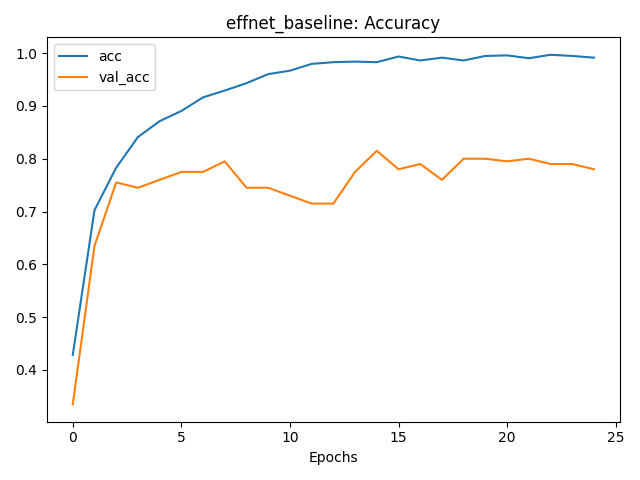
\includegraphics[width=0.48\textwidth]{../new_work/figures/effnet_baseline_acc.png}
  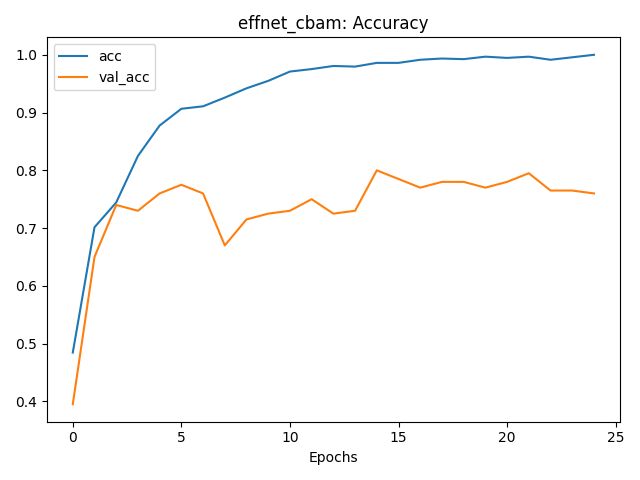
\includegraphics[width=0.48\textwidth]{../new_work/figures/effnet_cbam_acc.png}\\
  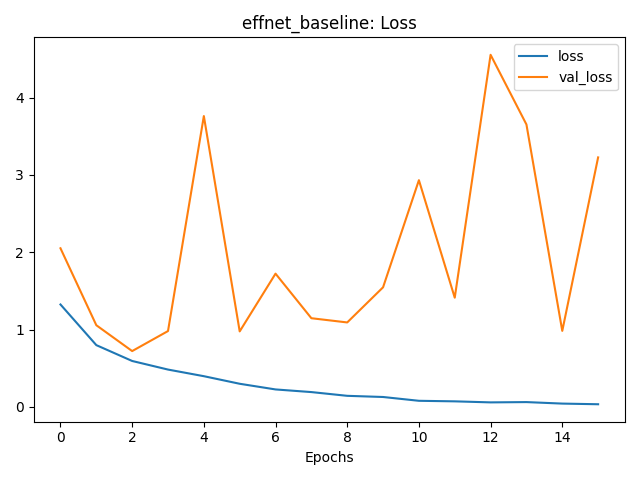
\includegraphics[width=0.48\textwidth]{../new_work/figures/effnet_baseline_loss.png}
  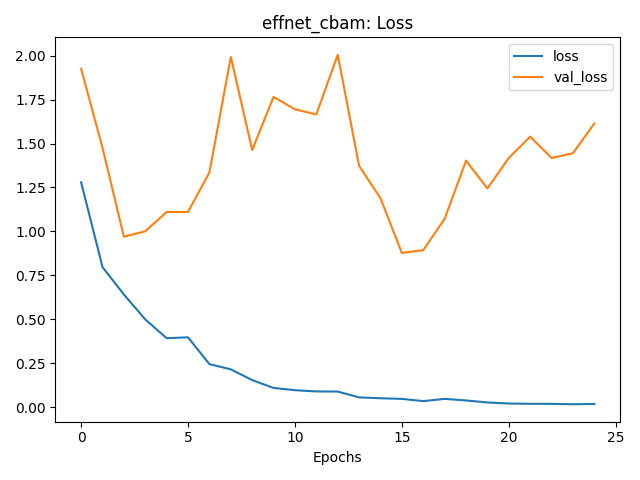
\includegraphics[width=0.48\textwidth]{../new_work/figures/effnet_cbam_loss.png}
  \caption{Training dynamics: accuracy (top) and loss (bottom) for EfficientNet baseline (left) and EfficientNet+CBAM (right).}
  \label{fig:train_curves}
\end{figure}

\begin{figure}[t]
  \centering
  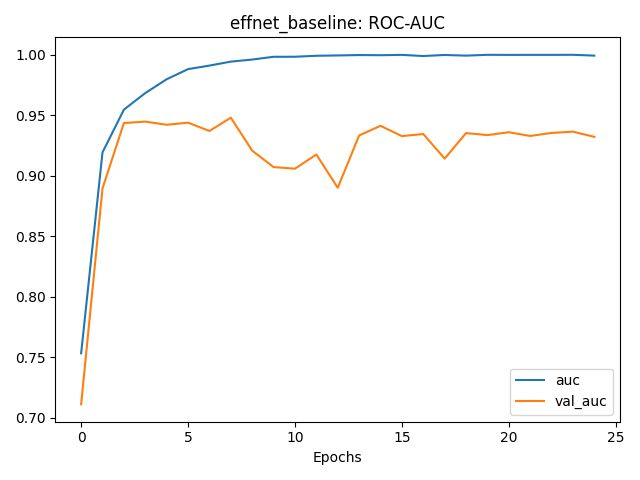
\includegraphics[width=0.48\textwidth]{../new_work/figures/effnet_baseline_auc.png}
  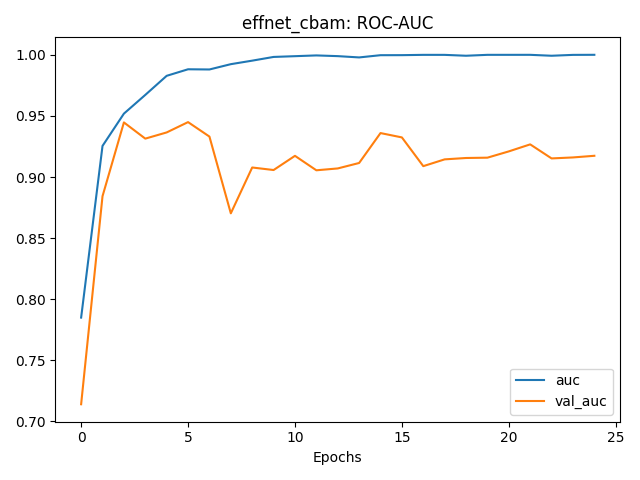
\includegraphics[width=0.48\textwidth]{../new_work/figures/effnet_cbam_auc.png}\\
  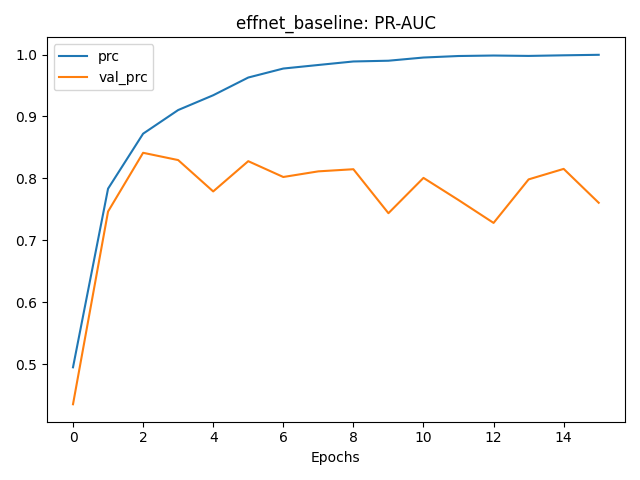
\includegraphics[width=0.48\textwidth]{../new_work/figures/effnet_baseline_prc.png}
  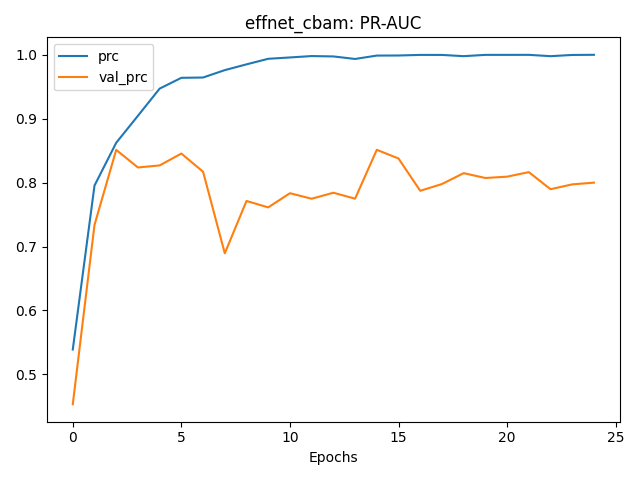
\includegraphics[width=0.48\textwidth]{../new_work/figures/effnet_cbam_prc.png}
  \caption{AUC metrics: ROC\textendash AUC (top) and PR\textendash AUC (bottom) for baseline (left) and CBAM (right).}
  \label{fig:auc_curves}
\end{figure}

\begin{figure}[t]
  \centering
  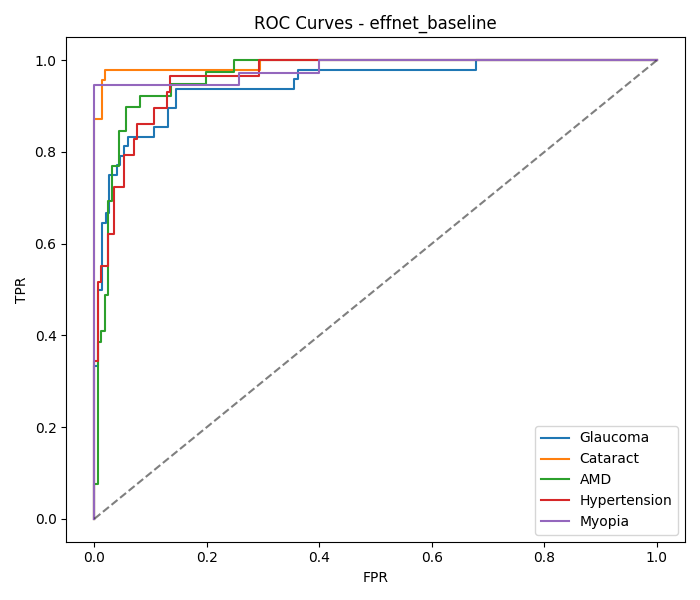
\includegraphics[width=0.48\textwidth]{../new_work/figures/roc_curves_effnet_baseline.png}
  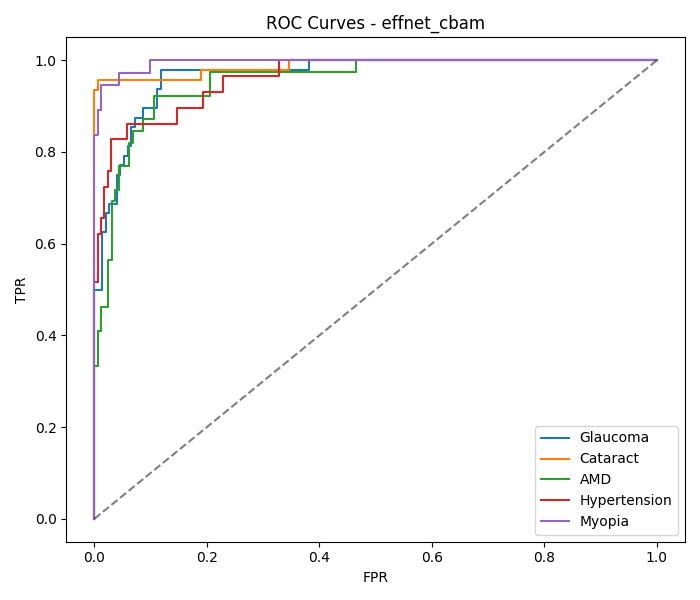
\includegraphics[width=0.48\textwidth]{../new_work/figures/roc_curves_effnet_cbam.png}\\
  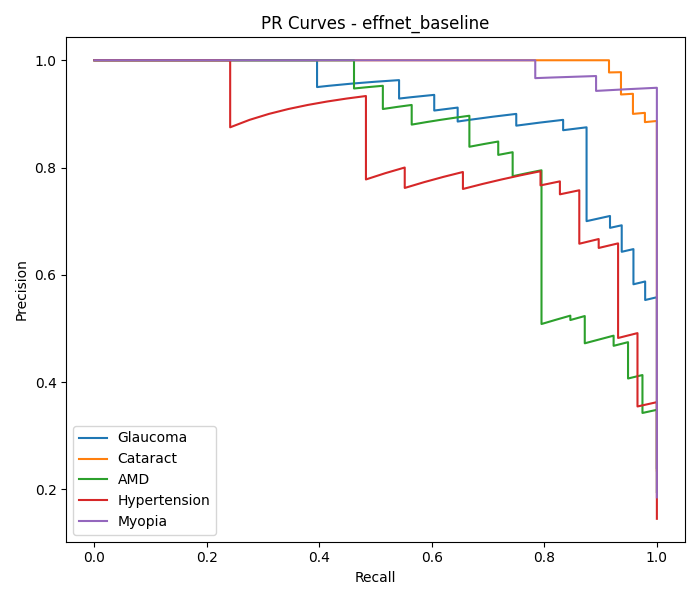
\includegraphics[width=0.48\textwidth]{../new_work/figures/pr_curves_effnet_baseline.png}
  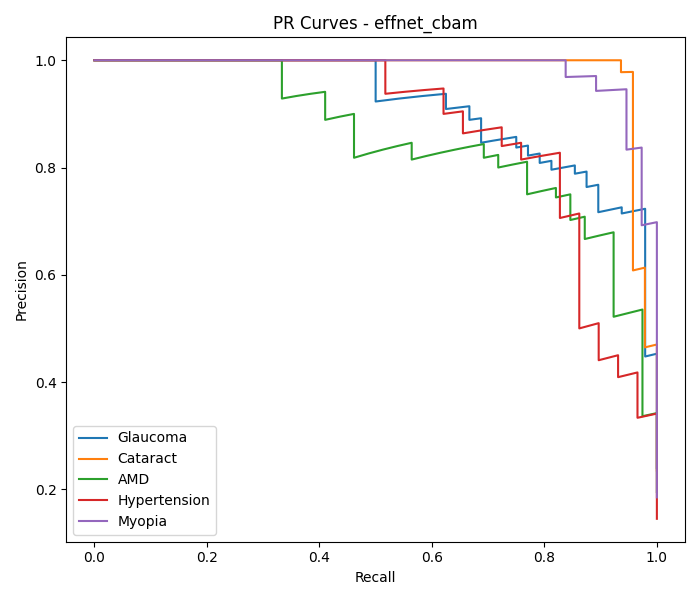
\includegraphics[width=0.48\textwidth]{../new_work/figures/pr_curves_effnet_cbam.png}
  \caption{Per\textendash class ROC (top) and PR (bottom) curves for baseline (left) vs. CBAM (right).}
  \label{fig:perclass_curves}
\end{figure}

\begin{figure}[t]
  \centering
  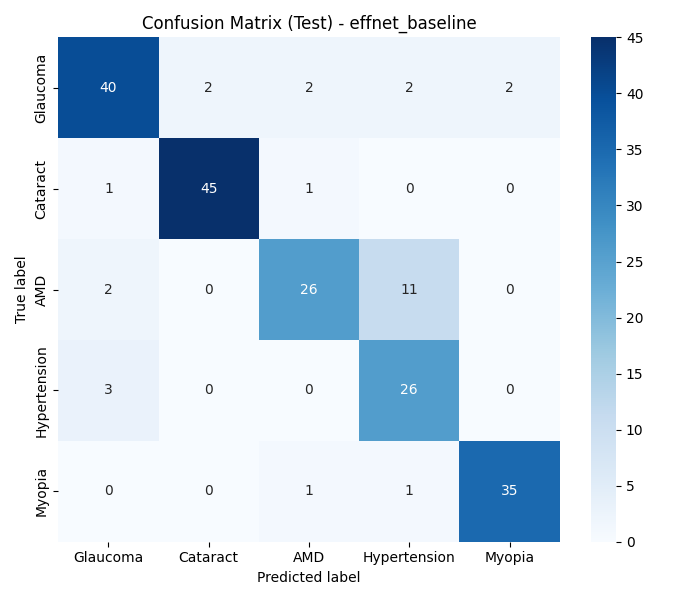
\includegraphics[width=0.48\textwidth]{../new_work/figures/cm_effnet_baseline_counts.png}
  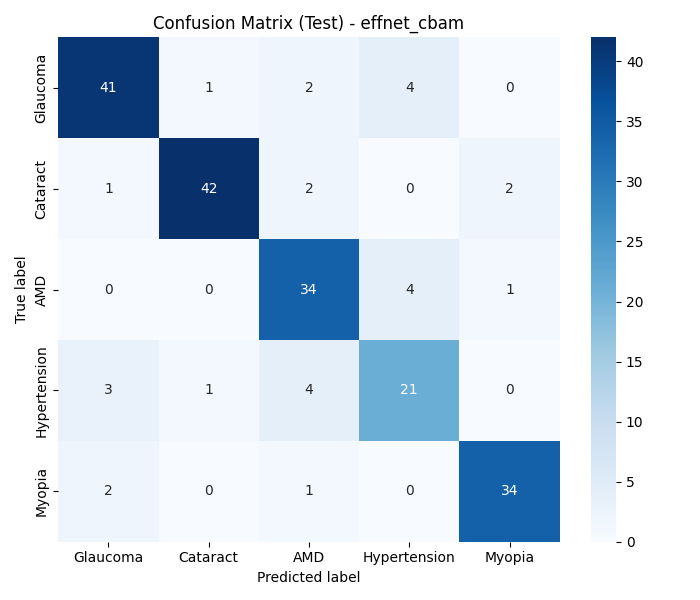
\includegraphics[width=0.48\textwidth]{../new_work/figures/cm_effnet_cbam_counts.png}
  \caption{Confusion matrices (counts) on the held\textendash out test set for baseline (left) and CBAM (right).}
  \label{fig:cms}
\end{figure}


% 7. Conclusion and Future Work
\chapter{Conclusion and Future Work}
We synthesize empirical findings and outline a forward path. The CBAM module consistently improved the EfficientNet baseline under identical conditions, especially for challenging classes. We discuss implications for clinical screening pipelines and propose targeted next steps.
We presented a practical comparison of an EfficientNet baseline and an EfficientNet+CBAM attention variant on ODIR\textendash 5K. Attention improved several classes, and the pipeline reliably exported artifacts for transparent analysis. Hypertension remains difficult in single\textendash label settings; future work will explore multi\textendash label training, better hypertension\textendash specific augmentation, and backbone scaling (B3+) to further improve macro F1.



% Acknowledgements (optional)
\section*{Acknowledgements}
We would like to thank our supervisor, \textbf{\supervisor}, for guidance and feedback throughout this project.



% References
\clearpage
\bibliographystyle{unsrtnat}
\bibliography{references}

\end{document}


